\documentclass{article}
\usepackage[T1]{fontenc}  
\usepackage[scaled=0.82]{beramono}  
\usepackage{microtype} 
\usepackage{amsmath}
\usepackage{amsfonts}
\usepackage{mathtools}
\usepackage{bm}
\usepackage{slashed}
\usepackage{amssymb}
\usepackage{hyperref}
\usepackage{nameref}
\usepackage{siunitx}
\usepackage{mhchem}
\usepackage{subcaption}
% \usepackage[backend=bibtex]{biblatex}
\usepackage[margin=2cm]{geometry}
% \addbibresource{matching-pursuit.bib}

\DeclareMathOperator{\E}{E}

\title{Study on MCP-PMT longtail based on secondary electron emission}
% \title{MCP reasearch}
\author{Jun,Weng; Zhang, Aiqiang; Xu, Benda;} %\\ Center for High Energy Physics}
\date{\today}

\begin{document}
\maketitle
\section{Introduction}\label{sec:Introduction}
\section{The long-tail in MCP-PMT charge response }\label{sec:long-tail}
\subsection{Single photoelectron charge response}\label{subsec:statistical}
When the photomultiplier is in operation, the light incident on the photocathode produces photoelectrons via the photoelectric effect
which is a Poisson process. Then photoelectrons can be collected by the MCP under the influence of an electric field, which is a Bernoulli process.
MCP amplifies a single collected  electron, and when the amplification is large enough (usually more than 100 times),
the resulting charge follows a Gaussian distribution $\mathcal{N} (Q_1, \sigma_1^2)$. When multiple electrons are collected at the same time, the resulting charge
distribution is the sum of the charges generated by the amplification of multiple single electrons,
which can still be described by the Gaussian distribution $\mathcal{N} (nQ_1, n\sigma_1^2)$.
The charge response of MCP-PMTS can be discribed as \refeq{eq:sreal}~\cite{1994Absolute}
\begin{equation}
    \begin{aligned}
        Q_{ideal} & = P(n;\mu)\bigotimes G_n(x;nQ_1,\sqrt{n}\sigma_1)                                                                      \\
                  & =\sum_{n = 0}^{\infty}\frac{\mu^n e^{-\mu}}{n!}\frac{1}{\sigma_1\sqrt{2\pi n}}\exp(-\frac{{(x-nQ_1)}^2}{2n\sigma_1^2})
    \end{aligned}
    \label{eq:sreal}
\end{equation}
$\mu$ is the mean number of photoelectrons collected by MCP.\@ $P(n;\mu) = \frac{\mu^n e^{-\mu}}{n!}$ is the probability of $n$ photoelectrons obseved.

When $\mu$ is less than 0.1, the probability of observing two or more photoelectrons is less than one tenth of the probability
of observing one photoelectron, and the PMT charge response is left with two Gaussian peaks as Fig~\ref{fig:spe_sreal}
which is supposed to be SPE spectrum with pedestal peak($Q=0$) and single PE peak($Q=Q_1$)\cite{Xia_2015}.
\begin{figure}[ht]
    \centering
    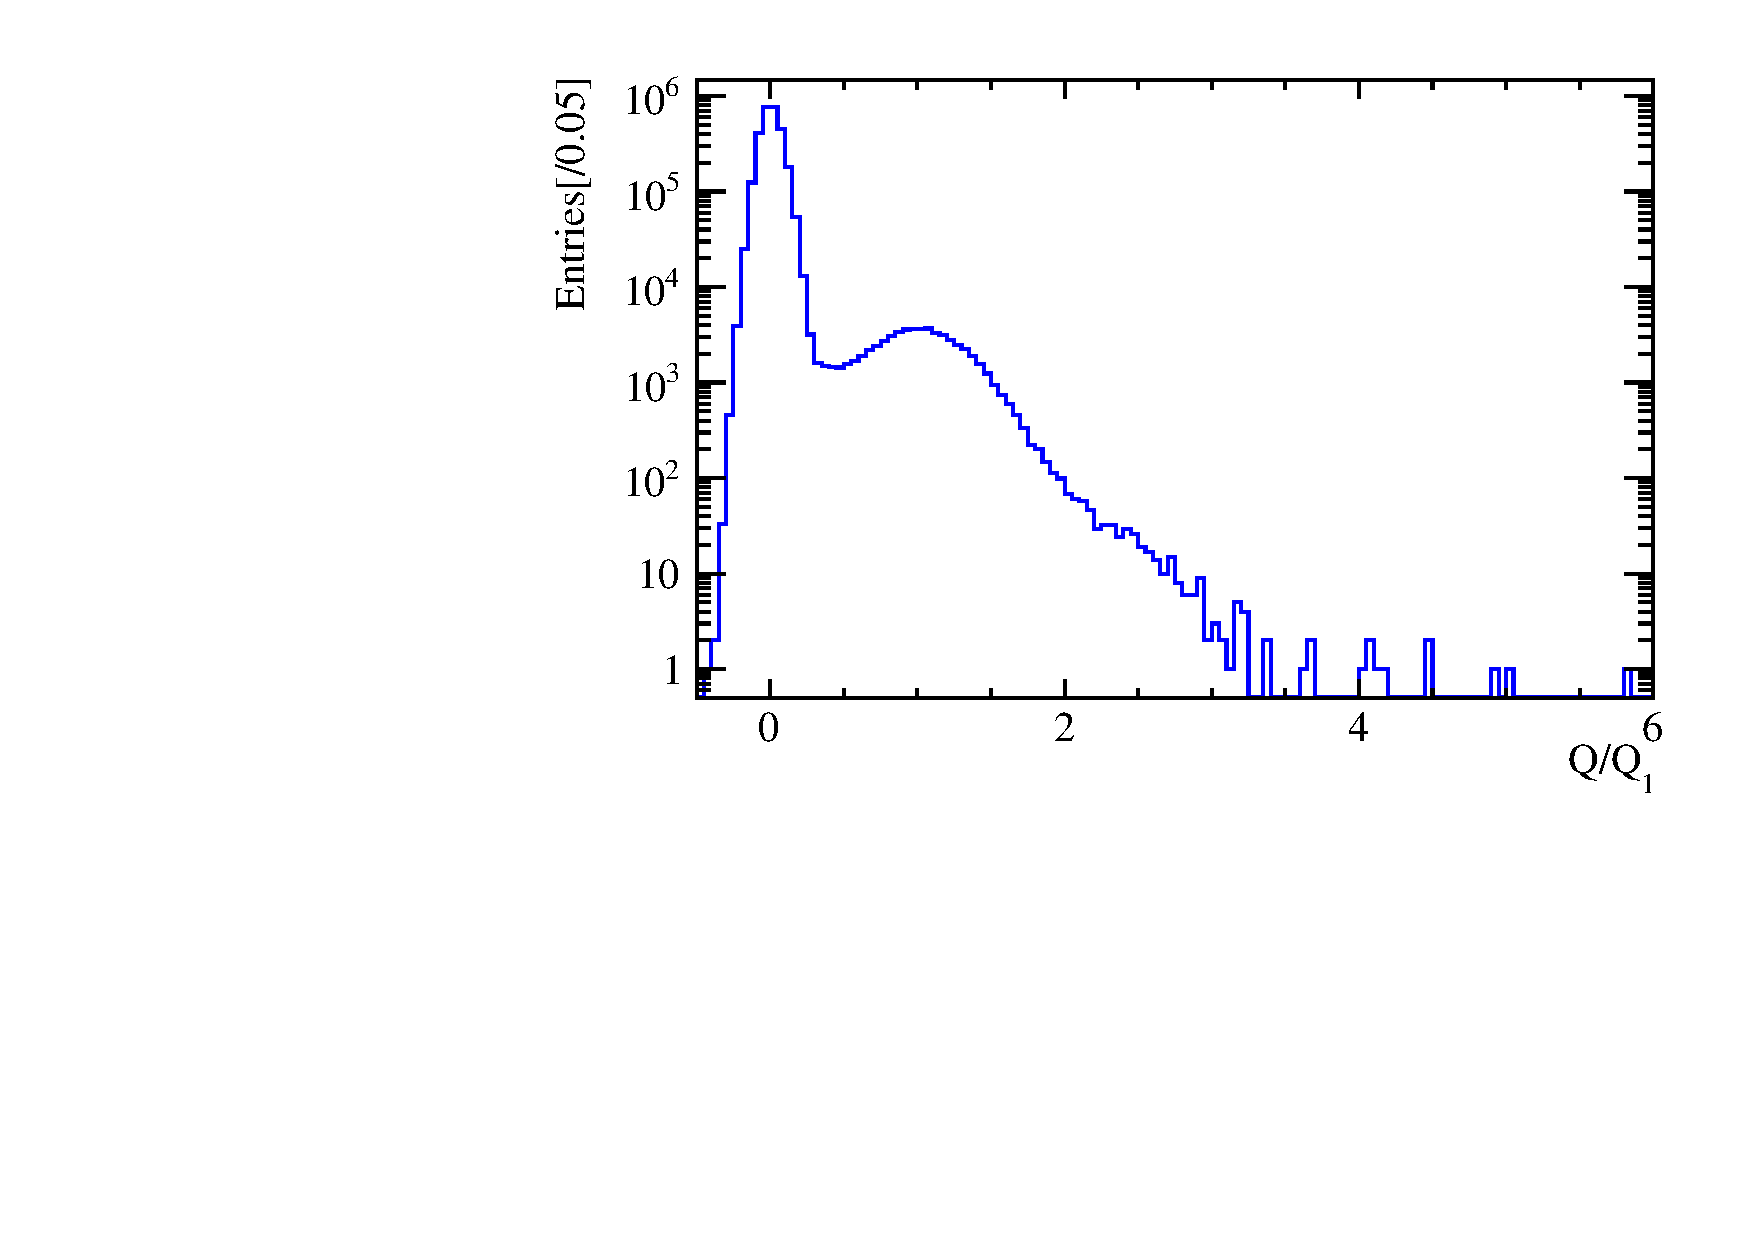
\includegraphics[height=7cm]{pic/siglepe.pdf}
    \caption{Single photoelectron charge response of Hamamatsu CR365}
    \label{fig:spe_sreal}
\end{figure}
\subsection{long tail in MCP-PMT charge response}\label{subsec:tail}
In the performance tests to evaluate MCP-PMT used by JNE, we found a long tail in the charge spectrum of MCP-PMTS in the single photoelectron mode as shown in Fig~\ref{fig:tail}
\begin{figure}[ht]
    \centering
    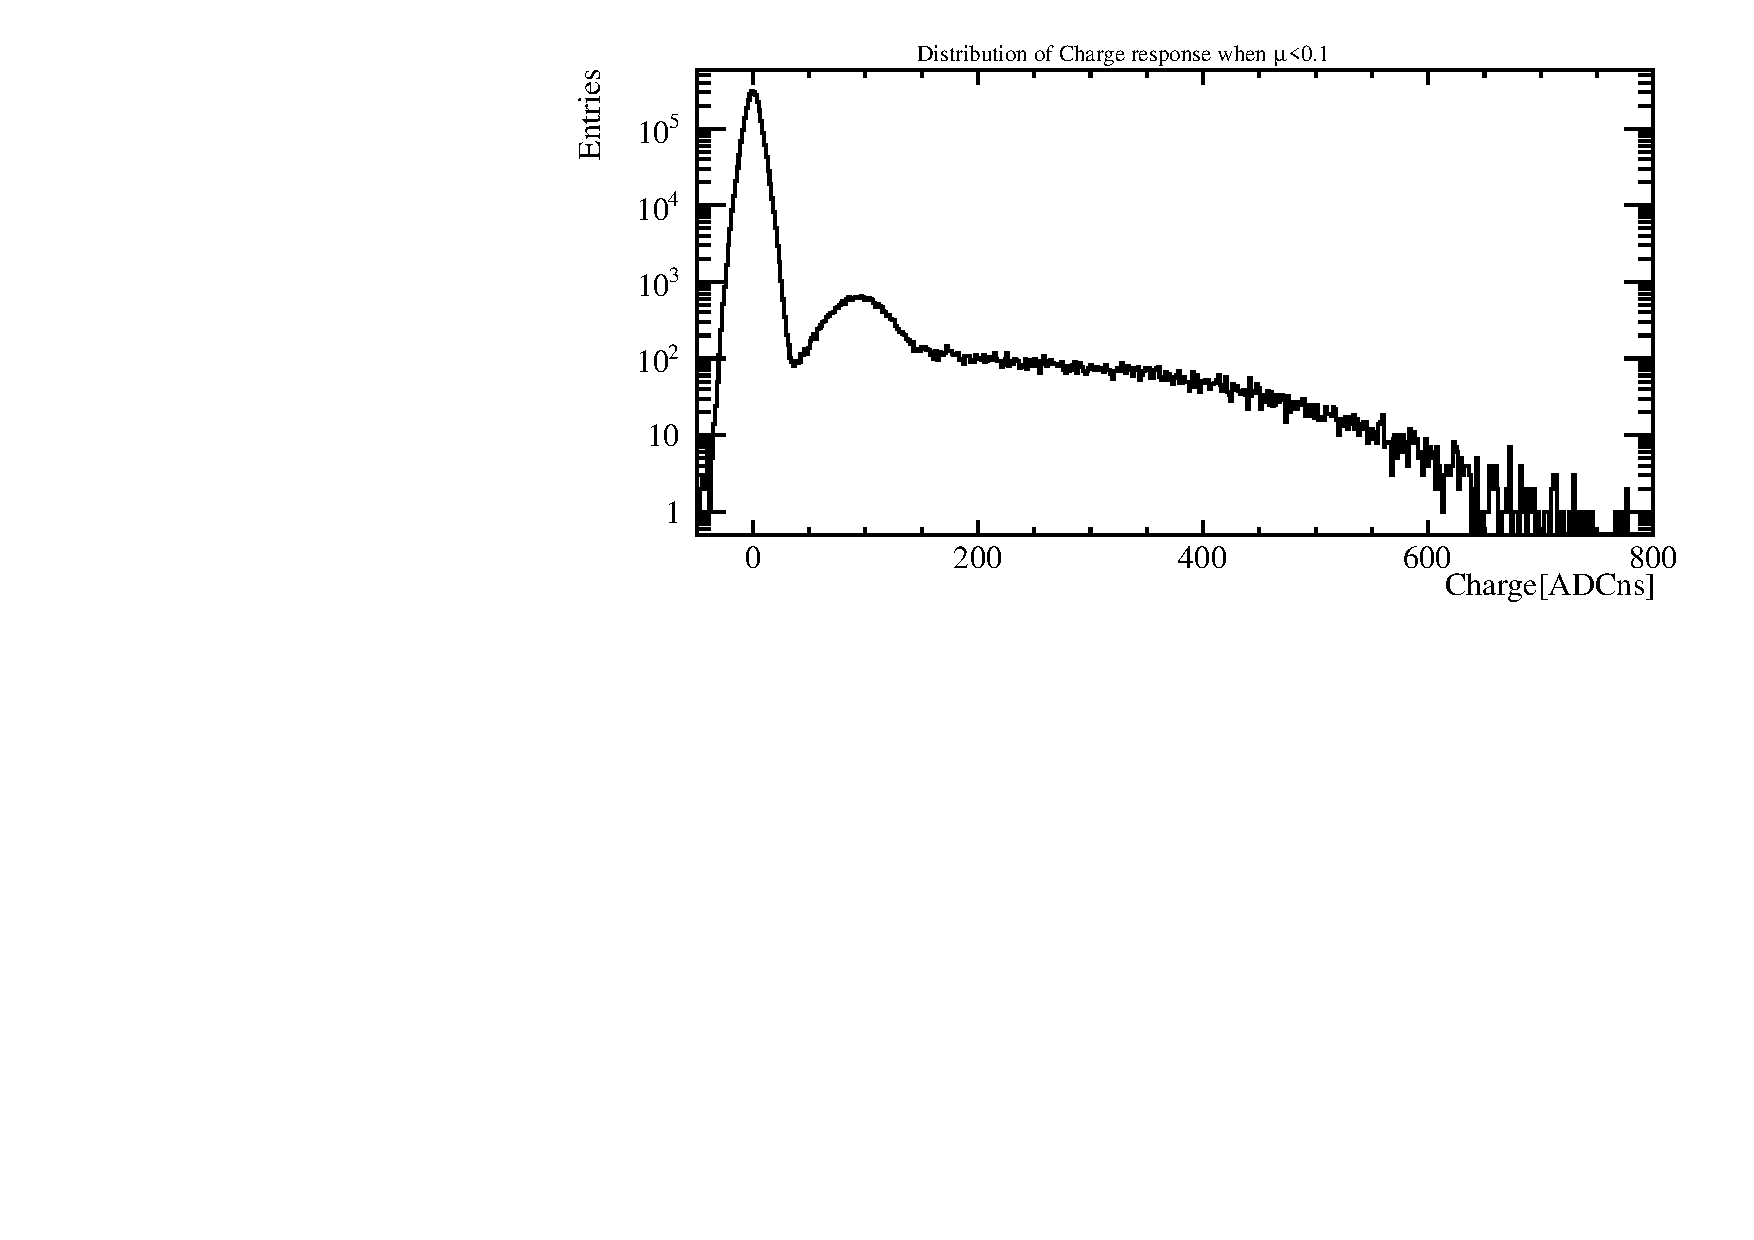
\includegraphics[height=7cm]{pic/longtail.pdf}
    \caption{Single photoelectron charge response of MCP-PMT PM2112$-$9089F}\label{fig:tail}
\end{figure}
\section{Statistical model of MCP-PMT charge response}
\subsection{The structure of MCP-PMT}\label{subsec:structure}
When the photon reaches the photocathode, it is converted into photoelectron through photoelectric conversion
Under the influence of electric field, it reaches the microchannel plate~(MCP). The microchannel plate is coated
with secondary emission material of certain thickness. The electrons interact with the surface of the microchannel plate to generate multiple electrons.
These electrons interact with the surface of the microchannel plate continuously under the action of electric field to form multiple electrons.
Finally, they reach the anode to form electrical signals that can be directly measured.
\begin{figure}[ht]
    \centering
    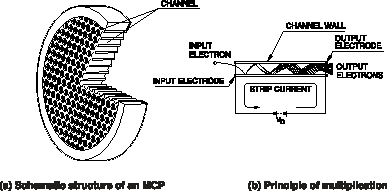
\includegraphics[height=5cm]{pic/structure.pdf}
    \caption{After entering the MCP channel, the electron collides with the channel wall for many times and multiplies in a cascade process}\label{fig:structure}
\end{figure}

In fact, when photoelectrons reach the upper surface of the MCP,
they may enter the MCP channel directly and undergo a cascade multiplication process,
which is described in Fig~\ref{fig:structure}.
It may also collide with the upper face of the MCP.\@
The photoelectron will not be amplified because of absorption process and so on.
The collection efficiency is then limited to the proportion of the open area of
the channel to the surface area of the MCP.\@

In order to improve the collection efficiency, it is necessary to make more photoelectrons observed.
The MCP upper surface of the MCP-PMTs used by JNE is coated with a layer of secondary emission material\cite{zzj2021Al}
called atomic layer deposition (ALD) technique which is used to improve the lifetime of the MCP-PMT
at first and  was later found to increase the found that the gain, the single electron resolution
and the peak-to-valley ratio of MCP-PMT \cite{2021Effects}.
\begin{figure}[ht]
    \centering
    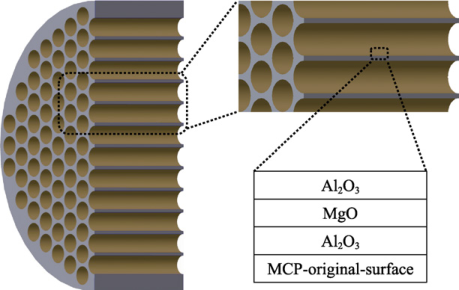
\includegraphics[height=5cm]{pic/ALD.pdf}
    \caption{$Al_2O_3/MgO/Al_2O_3$}\label{fig:A LD}
\end{figure}

Therefore, the electrons from the upper surface of MCP can also enter the MCP hole for multiplication
under the influence of electric field after the collision between photoelectrons and the upper surface of MCP.\@
This means that MCP-PMT can work in two modes, and each photoelectron can only be amplified in one of these modes.
We define the mode that directly enter the channel for multiplication as \textit{channel mode} and
the mode that enters the channel for multiplication after colliding with the upper surface as \textit{surface mode}.
\begin{figure}[ht]
    \centering
    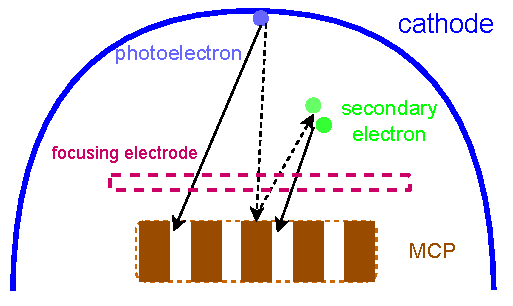
\includegraphics[height=5cm]{pic/MCPelectron.pdf}
    \caption{The photoelectrons directly enter the channel and enter the channels after hitting the upper face of the MCP}\label{fig:MCP}
\end{figure}
\subsection{double gamma model}\label{subsec:doublegamma}
Considering two multiplication modes, both of which multiply a single electron by a factor of $10^7$,
Their corresponding charge response can be described by Gaussian distribution respectively.
These two modes are mixed together in proportion to form the single photoelectronic response of MCP-PMTs as \refeq{eq:doublegaus}
\begin{equation}
    \label{eq:doublegaus}
    \begin{aligned}
         & Q_{MCP-PMT} = p\times Q_{channel\  mode} + (1-p)\times Q_{surface\  mode} \\
         & Q_{channel\  mode} \sim \mathcal{N} (\mu_1, \sigma_1)                     \\
         & Q_{surface\  mode} \sim \mathcal{N} (\mu_2, \sigma_2)
    \end{aligned}
\end{equation}
$p$ is proportional to the opening ratio of MCP, which can be understood as the probability that photoelectrons directly enter the MCP channel to multiply.
Use double Gaussian distribution to fit the charge response:
\begin{figure}[ht]
    \centering
    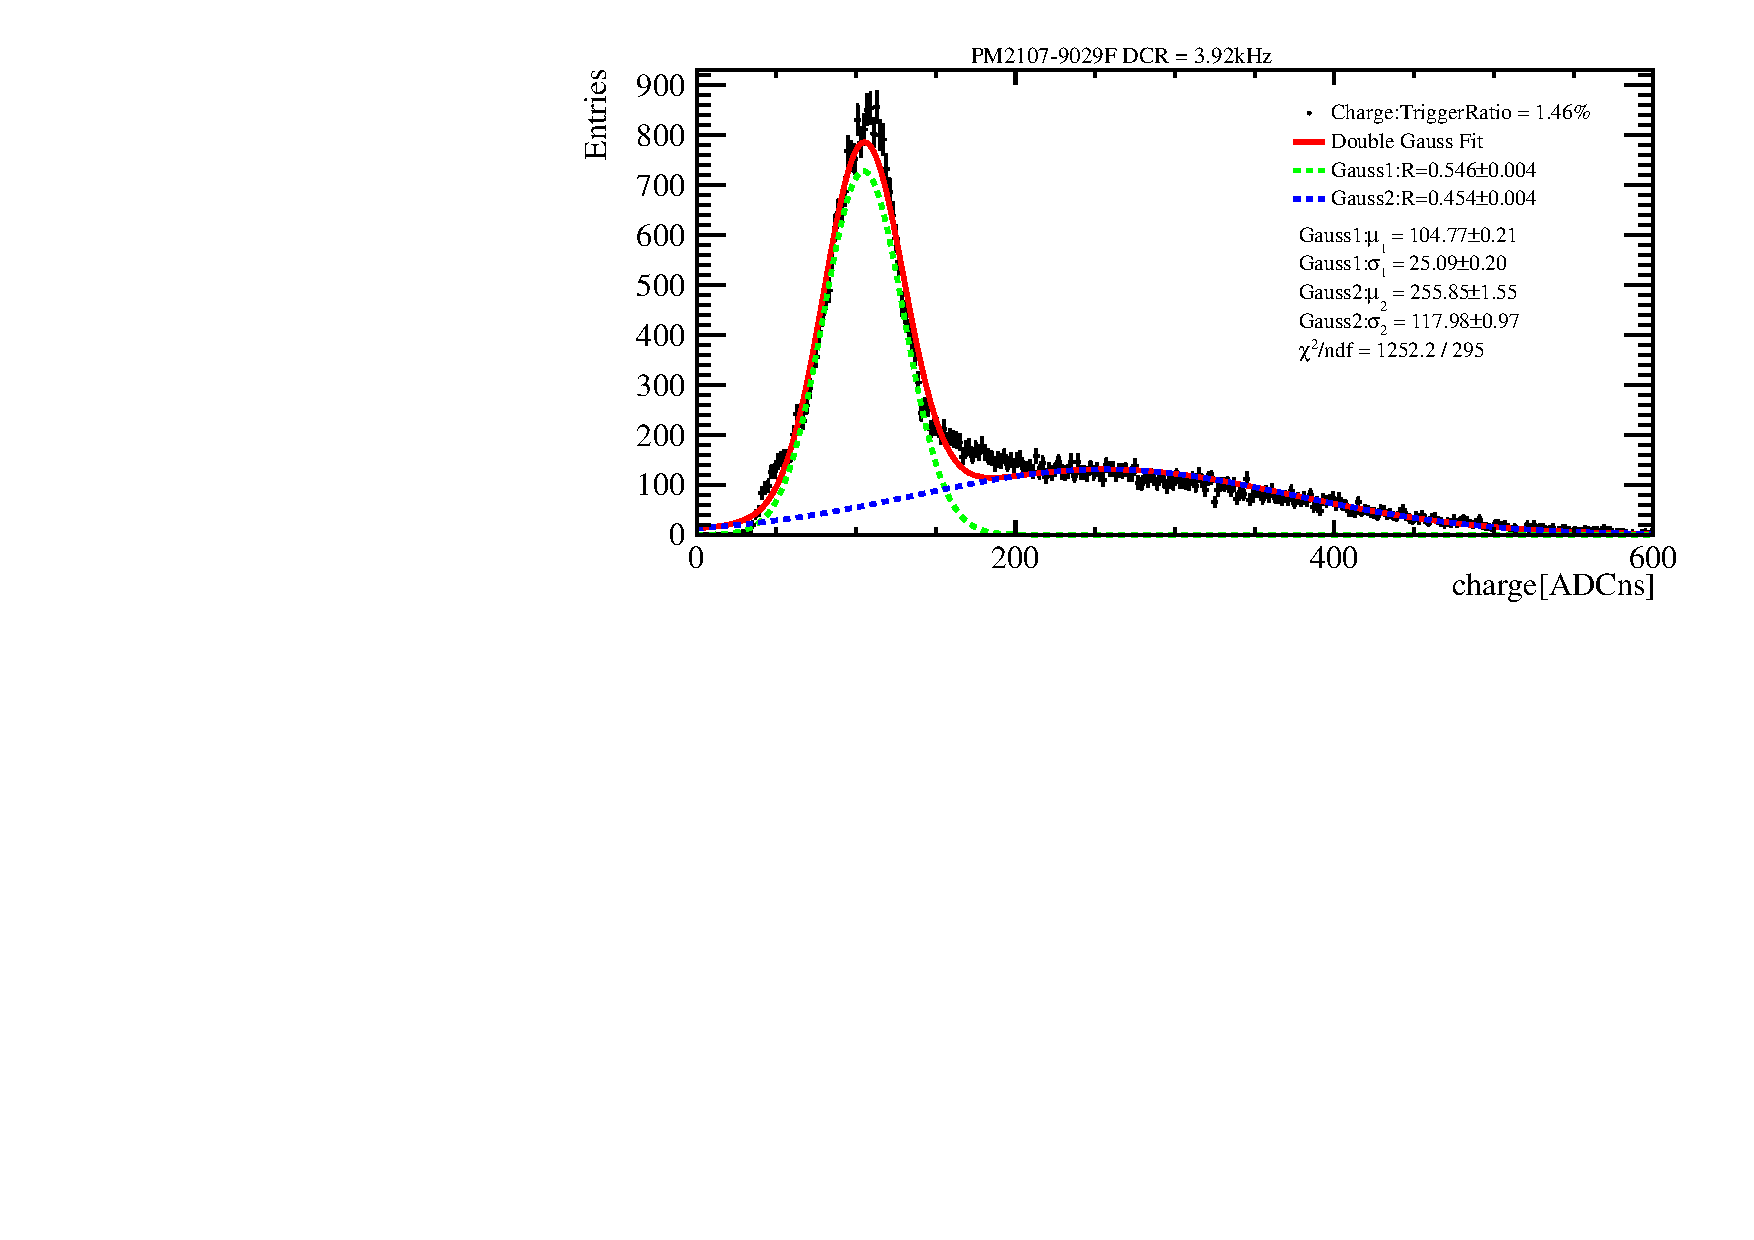
\includegraphics[height=5cm]{pic/doubleGauss.pdf}
    \caption{The proportion of \textit{channel mode} is bigger than \textit{surface mode}}\label{fig:doubleGauss}
\end{figure}

From~\ref{fig:doubleGauss}, there's still a probability when the charge is zero, which doesn't make physical sense.
In order to solve the problem, we introduce gamma distribution instead of Gaussian distribution.
The gamma distribution can be used to fit data with a Gaussian distribution, especially in certain situations,
such as when the data is skewed or non-negative. It is a good choise to discribe the charge spectrum of MCP-PMTs.
\begin{equation}
    \label{eq:gamma}
    \begin{aligned}
         & f(x ; \alpha, \beta)=\frac{x^{\alpha-1} e^{-\beta x} \beta^\alpha}{\Gamma(\alpha)} \quad \text { for } x>0 \quad \alpha, \beta>0 \\
         & \mu=\frac{\alpha}{\beta}                                                                                                         \\
         & \sigma^2=\frac{\alpha}{\beta^2}
    \end{aligned}
\end{equation}
$\alpha$ is the scale factor, $\beta$ is the rate factor and $\Gamma(\alpha)$ is the gamma function.
By adjusting the scale factor $\alpha$ and rate factor $\beta$, the mean and variance of the gamma distribution can be similar to the gauss distribution.
Using double gamma distribution as Eq~\ref{eq:doublegamma} to fit the charge spectrum of MCP-PMT as Fig~\ref{fig:doubleGamma}:
\begin{equation}
    \label{eq:doublegamma}
    \begin{aligned}
         & Q_{MCP-PMT} = p\times Q_{channel\  mode} + (1-p)\times Q_{surface\  mode} \\
         & Q_{channel\  mode} \sim \varGamma  (\alpha_1, \beta_1)                    \\
         & Q_{surface\  mode} \sim \varGamma  (\alpha_2, \beta_2)
    \end{aligned}
\end{equation}
\begin{figure}[ht]
    \centering
    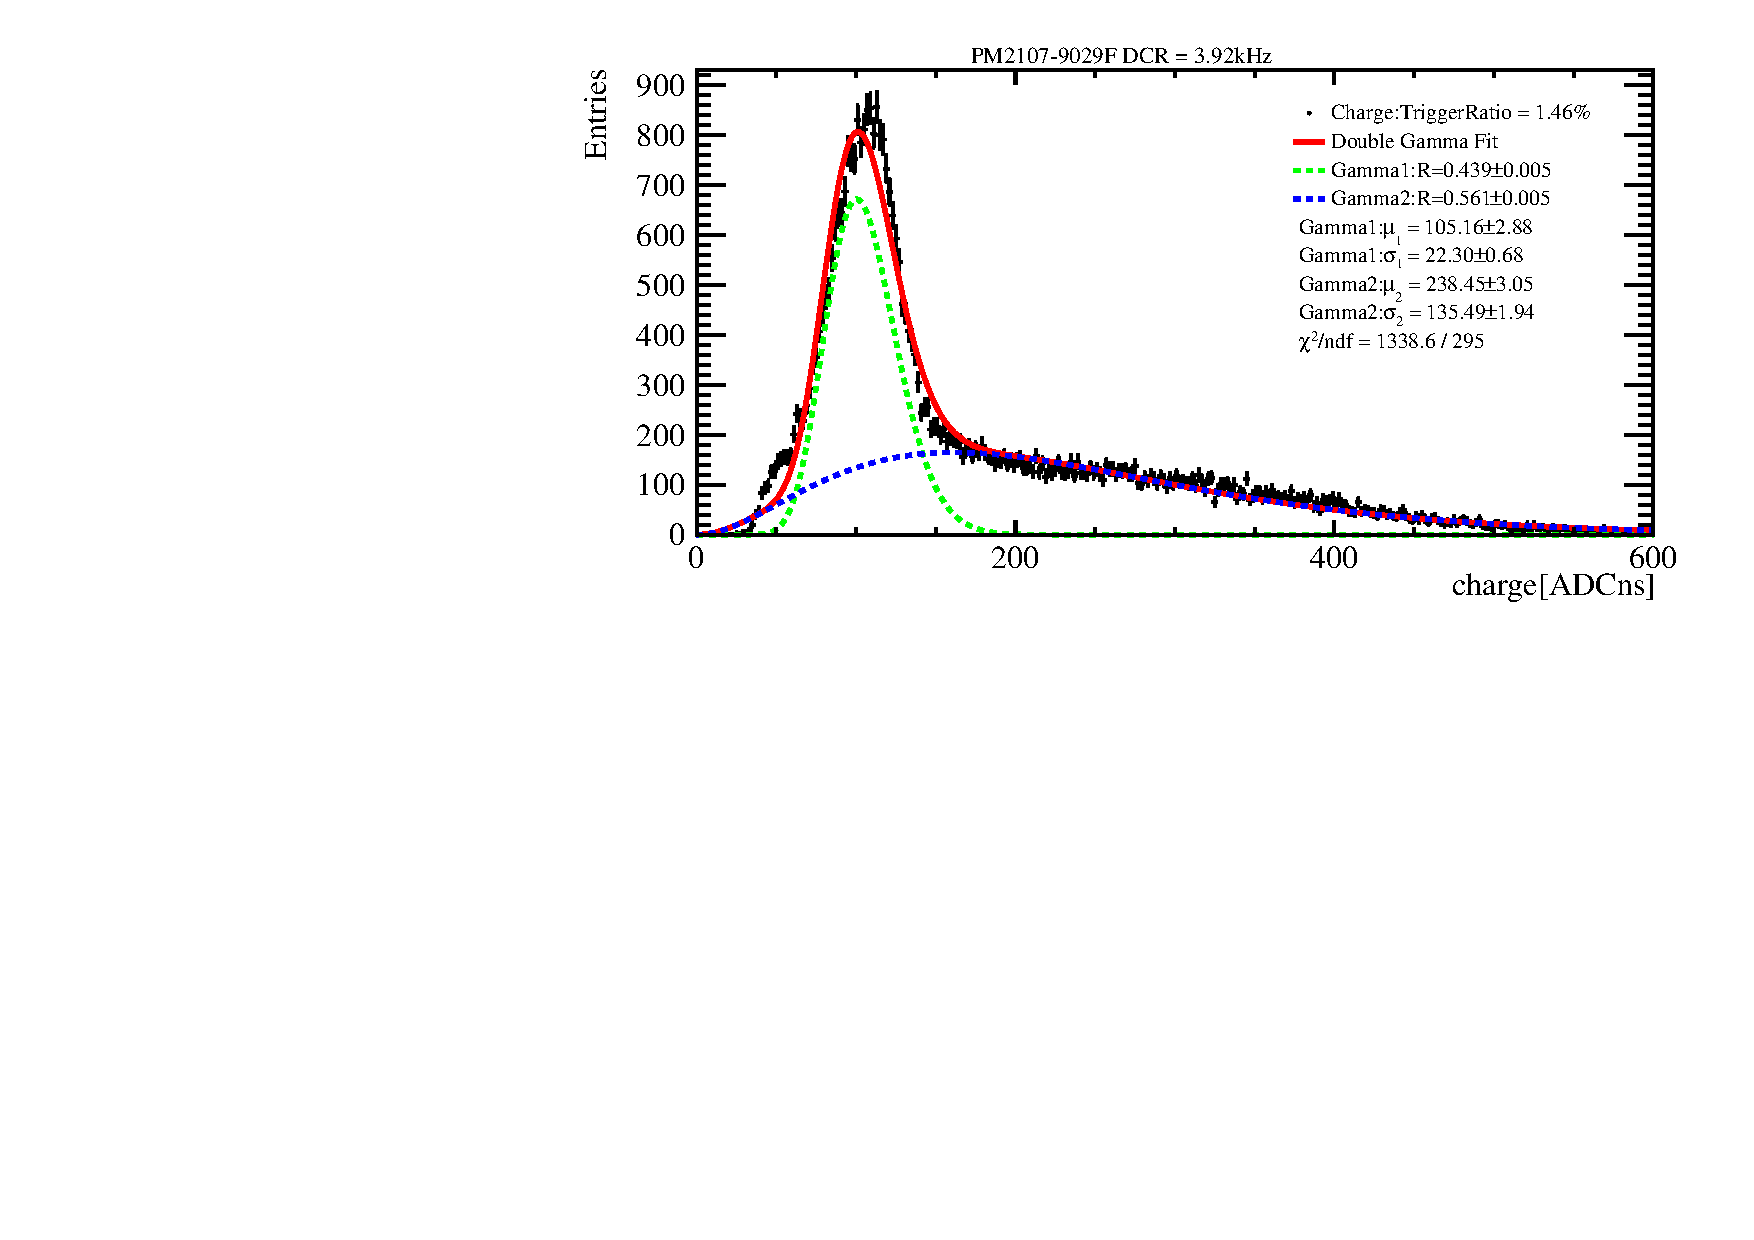
\includegraphics[height=5cm]{pic/doubleGamma.pdf}
    \caption{The proportion of \textit{channel mode} is bigger than \textit{surface mode}}\label{fig:doubleGamma}
\end{figure}
In double distribution fitting, the proportion $p$ is leass than 50\%, which is not consistent with the opening ratio of 0.65.
Also the chi-square value is not small enough to indicate the fitting is good enough.

\subsection{dark noise from MCP}\label{subsec:dnr}
The large chi-square value indicates that the fitting does not agree well with the SPE measured by experiment. We
found a small peak in $[30,50]$\si[]{ADCns} hypothesized due to dark noise. In MCP-PMT, there are three possible types of noise:
\begin{enumerate}
    \item {Dark noise (DR) mainly caused by the thermionic emission from the
          photocathode\cite{2019wenlj}}
    \item {After pulse caused by the ion feedback from the ionization of
          the residual gas or the amplification process\cite{2019wenlj}}
    \item {MCP noise caused by electron emission from the surface of the MCP}
\end{enumerate}
The first noise creates a charge response similar to that of a single photoelectron with random trigger time
and relatively small trigger rate. The second noise signal is related to the trigger signal of the light source,
the trigger rate of the light source, the greater the After pulse noise trigger rate.

We set the photocathode voltage to the same potential as the upper surface of the MCP, turn off the laser,
and test the dark noise from the MCP itself in the dark environment, get the  charge spectrum as~Fig\ref{fig:MCPDNR}:
\begin{figure}[ht]
    \centering
    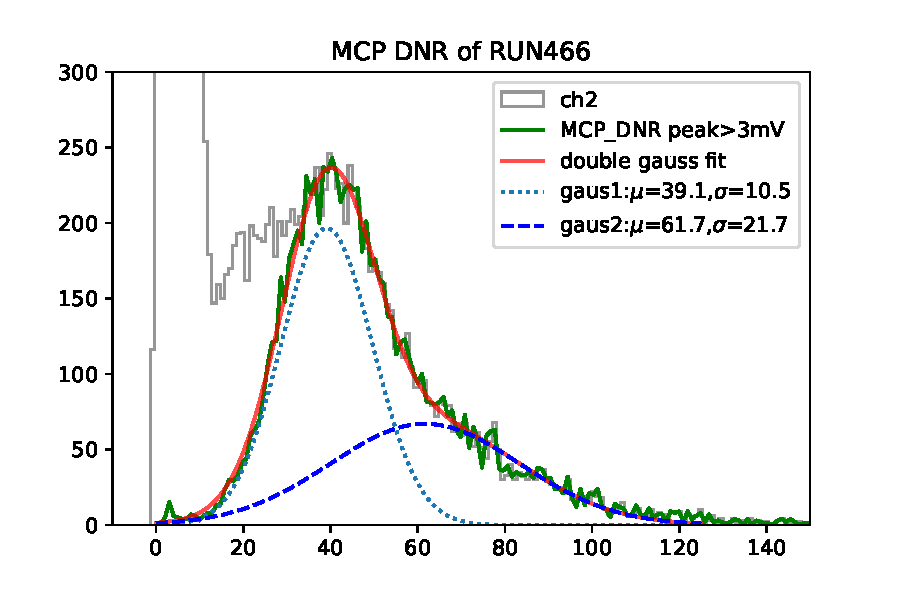
\includegraphics[height=5cm]{pic/MCP_DNR.pdf}
    \caption{Trigger ratio = 1.19\%}
    \label{fig:MCPDNR}
\end{figure}
MCP noise described by Gaussian  is considered in the fitting:
\begin{figure}[ht]
    \centering
    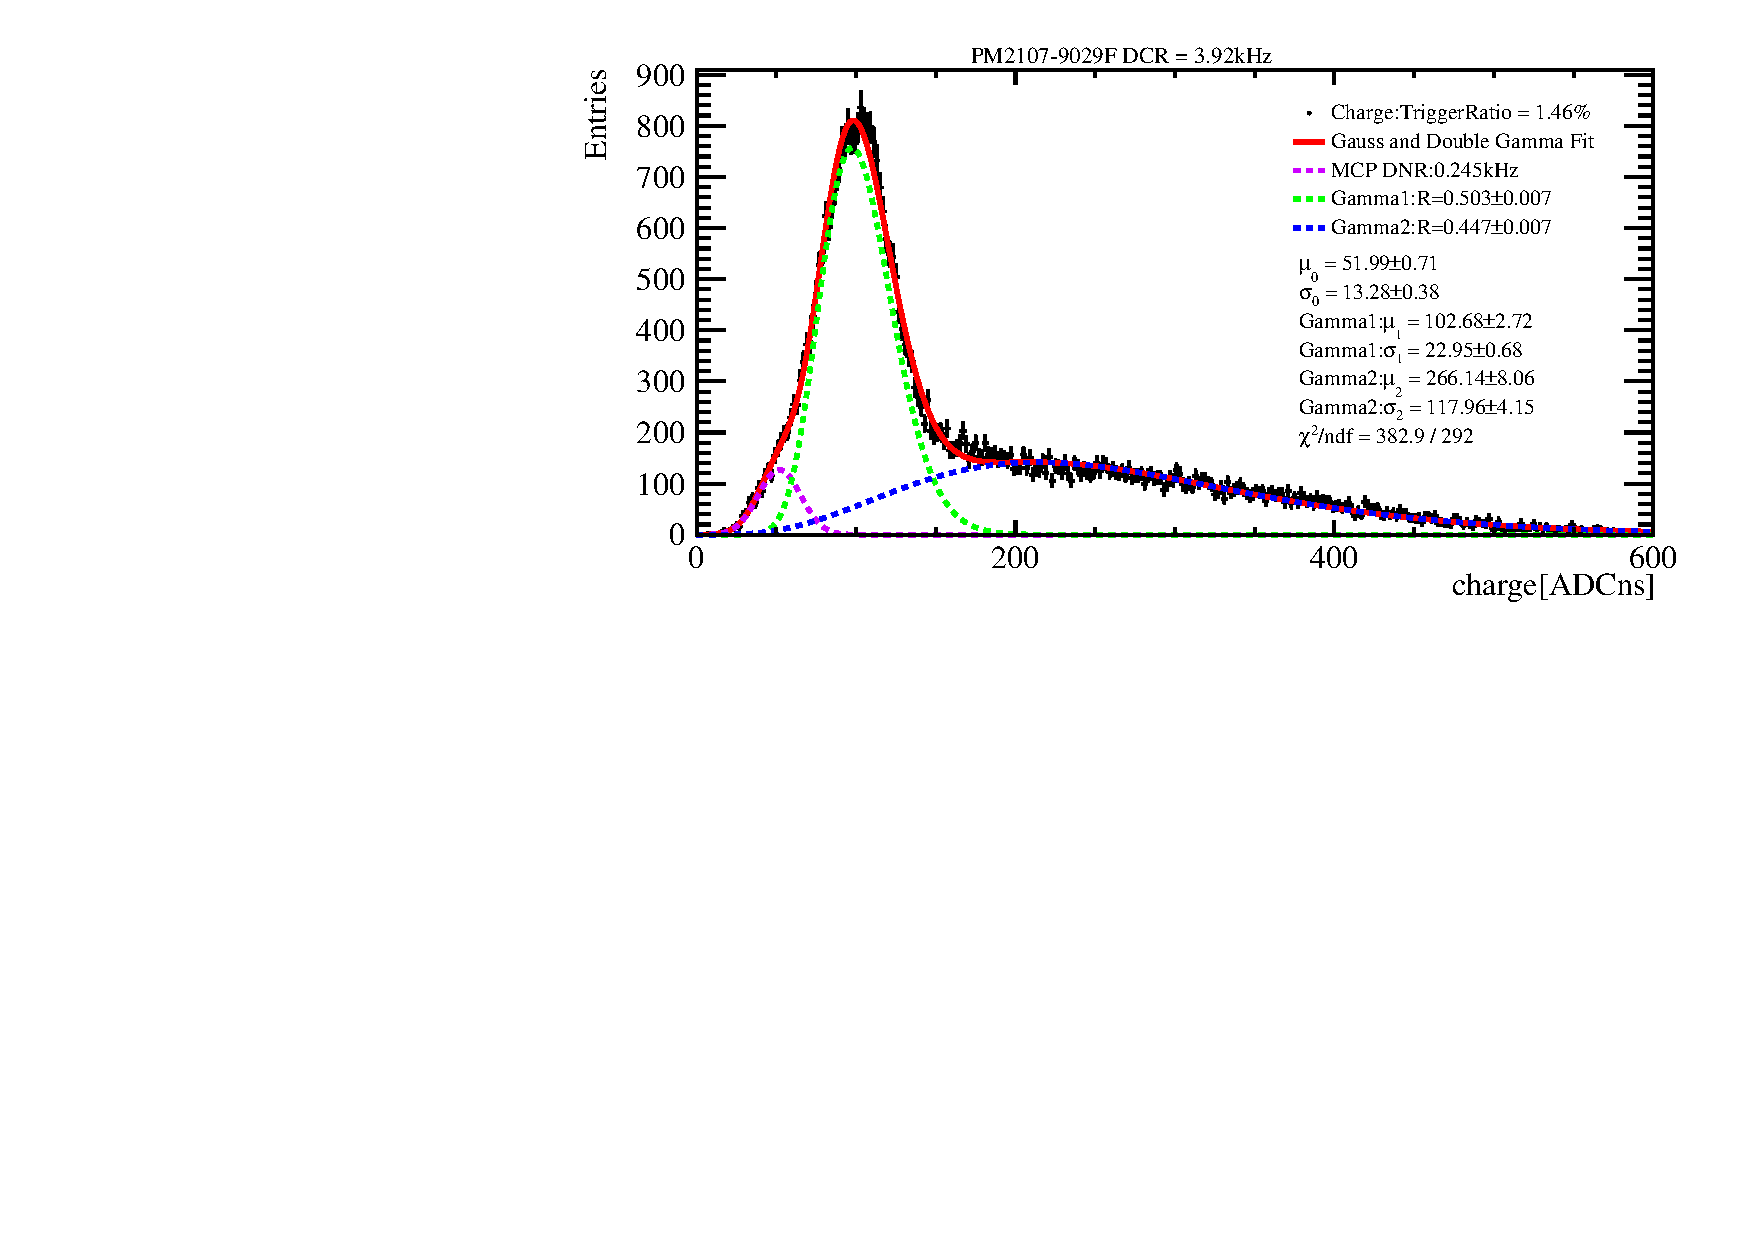
\includegraphics[height=5cm]{pic/gaussDgamma.pdf}
    \caption{Dark noise count rate (DCR) is \SI{3.92}{kHz} and dark noise count rate from MCP(MCP DNR) is \SI{0.245}{kHz}}\label{fig:gausDgam}
\end{figure}
\section{long tail based on secondary electron emission}\label{sec:see}


%\subsection{secondary electron emission}\label{subsec:fuman}
%Secondary electron emission (SEE) is a phenomenon in which an incident particle, such as an electron or ion, 
%collides with a solid surface and ejects one or more secondary electrons from the surface. 
%The secondary electrons are emitted due to the transfer of energy from the incident particle to the surface atoms, 
%which causes the ejection of electrons from the surface.
%SEE is an important physical process in many areas of science and technology, 
%including plasma physics, materials science, and microelectronics. In plasma physics, 
%SEE plays a critical role in determining the behavior of plasmas in contact with solid surfaces.
%In materials science, SEE is a key factor in determining the performance of materials under high-energy particle irradiation. 
%In microelectronics, SEE can cause damage to electronic devices and affect their performance.
%The magnitude of SEE depends on a variety of factors, including the energy and angle of incidence of the incident particle, 
%the composition and structure of the surface material, and the presence of surface contaminants. 
%In order to understand and predict the behavior of SEE, a variety of theoretical and experimental approaches have been developed, 
%including Monte Carlo simulations, analytical models, and experimental measurements.
\subsection{secondary electron energy spectrum}\label{subsec:fuman}
Secondary electron emission (SEE) is a phenomenon in which an incident particle, such as an electron or ion,
collides with a solid surface and ejects one or more secondary electrons from the surface.
The energy of secondary electrons is related to the initial energy of incident particle, incident Angle, target material and so on.
It is a complex energy distribution.
Since the energy of photoelectrons when produced by the photocathode is very low, only a few \SI{}{eV},
the energy of the photoelectron incident on the MCP is almost determined by the potential difference
between the photocathode and the MCP.\@ It is right to calcute the energy by analyzing the voltage divider circuit and the result is \SI{550}{eV} (to be determined).
The energie distribution of the secondary electrons (SES) can be discribed by using Furman self-consistent probabilistic model~\cite{2002Probabilistic}
when the incident energy is \SI{600}{eV} as Fig~\ref{fig:tail}.
What is equally important is how many secondary electrons can be produced at this incident energy,
which is also given the corresponding distribution in Fuman mpdel\cite{2002Probabilistic} as Fig~\ref{fig:secondaryelectron}
as SEY (secondary electron emission yield).

\begin{figure}[htbp]
    \centering
    \begin{subfigure}[b]{0.45\textwidth}
        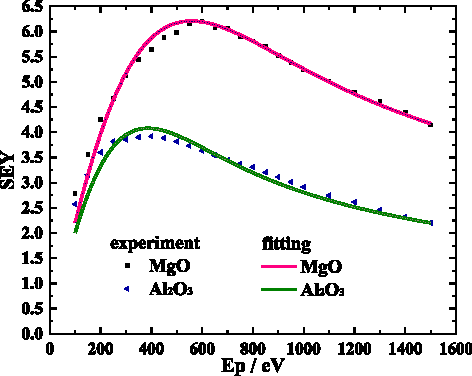
\includegraphics[width=\textwidth]{pic/SEE.pdf}
        \caption{secondary electron emission yield (SEY)}
        \label{fig:SEY}
    \end{subfigure}
    \begin{subfigure}[b]{0.45\textwidth}
        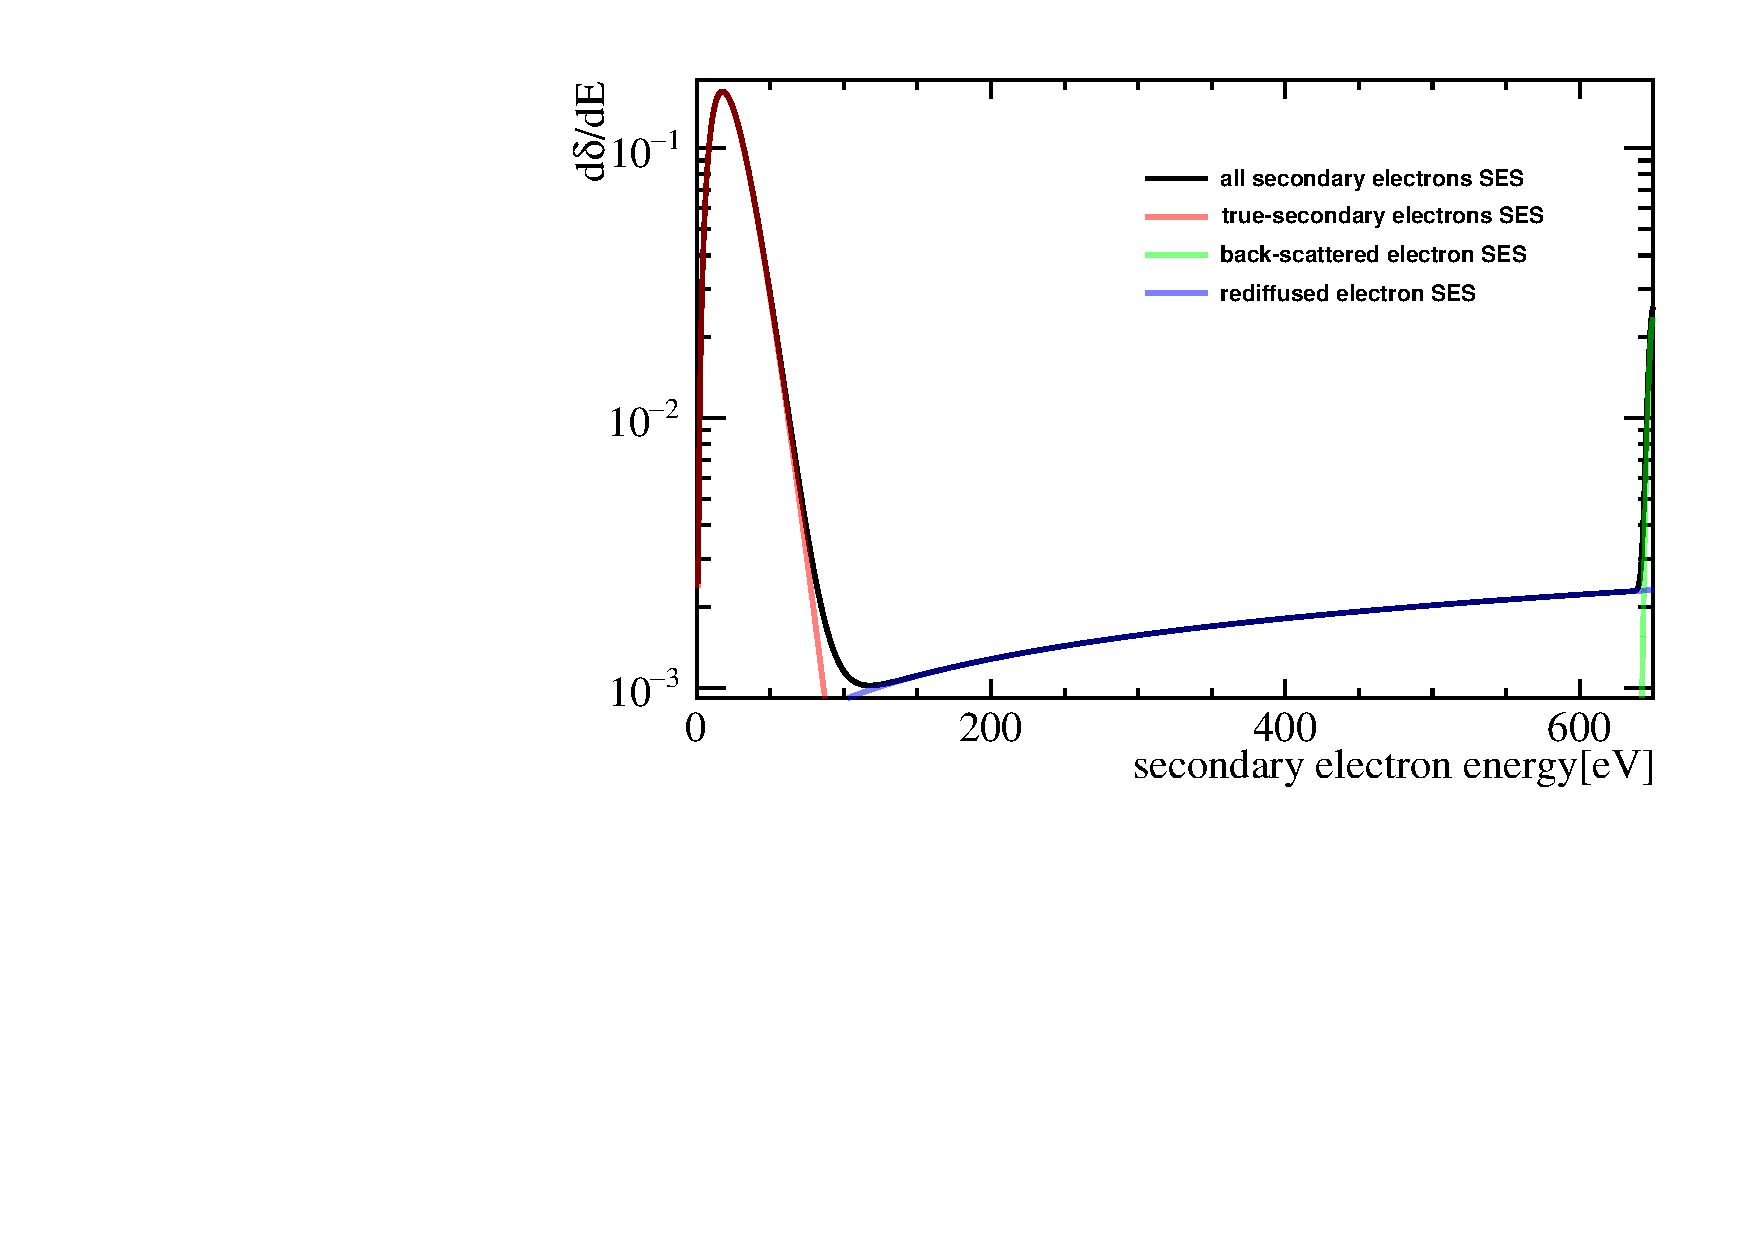
\includegraphics[width=\textwidth]{pic/SES.pdf}
        \caption{SES of secondary electrons when primary energy is \SI{600}{eV}}
        \label{fig:SES}
    \end{subfigure}
    \caption{SEE and SES of MCP}
    \label{fig:secondaryelectron}
\end{figure}


\subsection{Gain at low incident energy}\label{sec:gain}
\subsubsection{Experimental setup}
From Sec~\ref{subsec:fuman} and Fig~\ref{fig:secondaryelectron},
the energy of secondary emission electrons is less than the energy of primary electrons and
they are small and usually less than \SI{100}{eV}.
When the initial energy is below \SI{100}{eV}, the SEY is small,
which means that the secondary emission electrons generated on the upper surface of the MCP
do not multiply into the channel the same as the photoelectrons directly into the channel,
and the amount of charge gained may be lower. It is necessary to measure the relationship between the gain of MCP
and the initial energy of electrons.
\begin{figure}[ht]
    \centering
    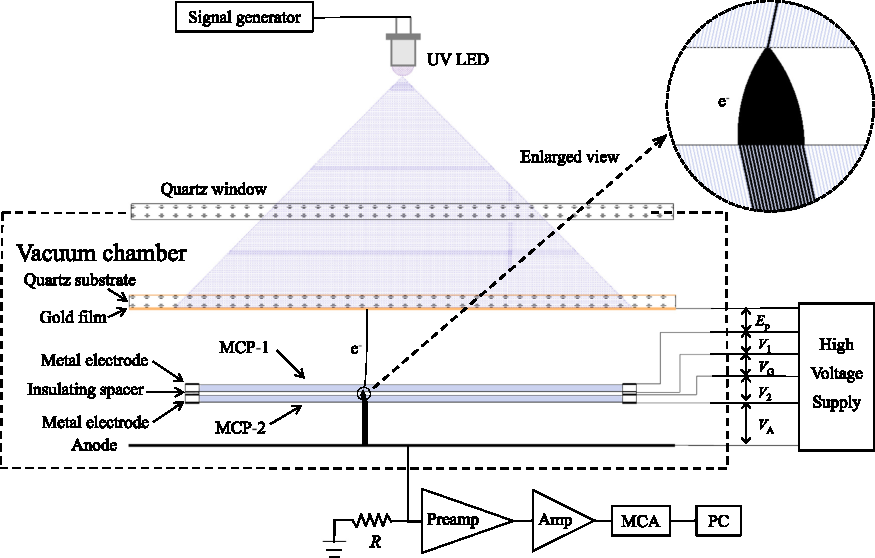
\includegraphics[width=0.6\textwidth]{pic/gain_ep_exp.pdf}
    \caption{Experimental setting}\label{fig:gain_exp}
\end{figure}
By adjusting the voltage of the power supply in the Fig~\ref{fig:gain_exp},
we separately set a stable and constant voltage difference at both ends of MCP to keep the electric field of MCP unchanged.
At the same time, the energy of electrons entering the upper surface of the MCP can be adjusted by
adjusting the potential difference between the photocathode and the upper surface of the MCP.
\subsubsection{Waveform analysis}
In order to avoid the deviation caused by waveform analysis, fsmp waveform analysis method is used in this paper.
\subsubsection{Experimental result}
In order to exclude the influence of surface secondary electron emission,
we did the same test on MCP-PMT with ALD coating and MCP-PMT without ALD coating,
and obtained the relationship of gain and electron energy as Fig~\ref{fig:gaintest}:
\begin{figure}[htbp]
    \centering
    \begin{subfigure}[b]{0.45\textwidth}
        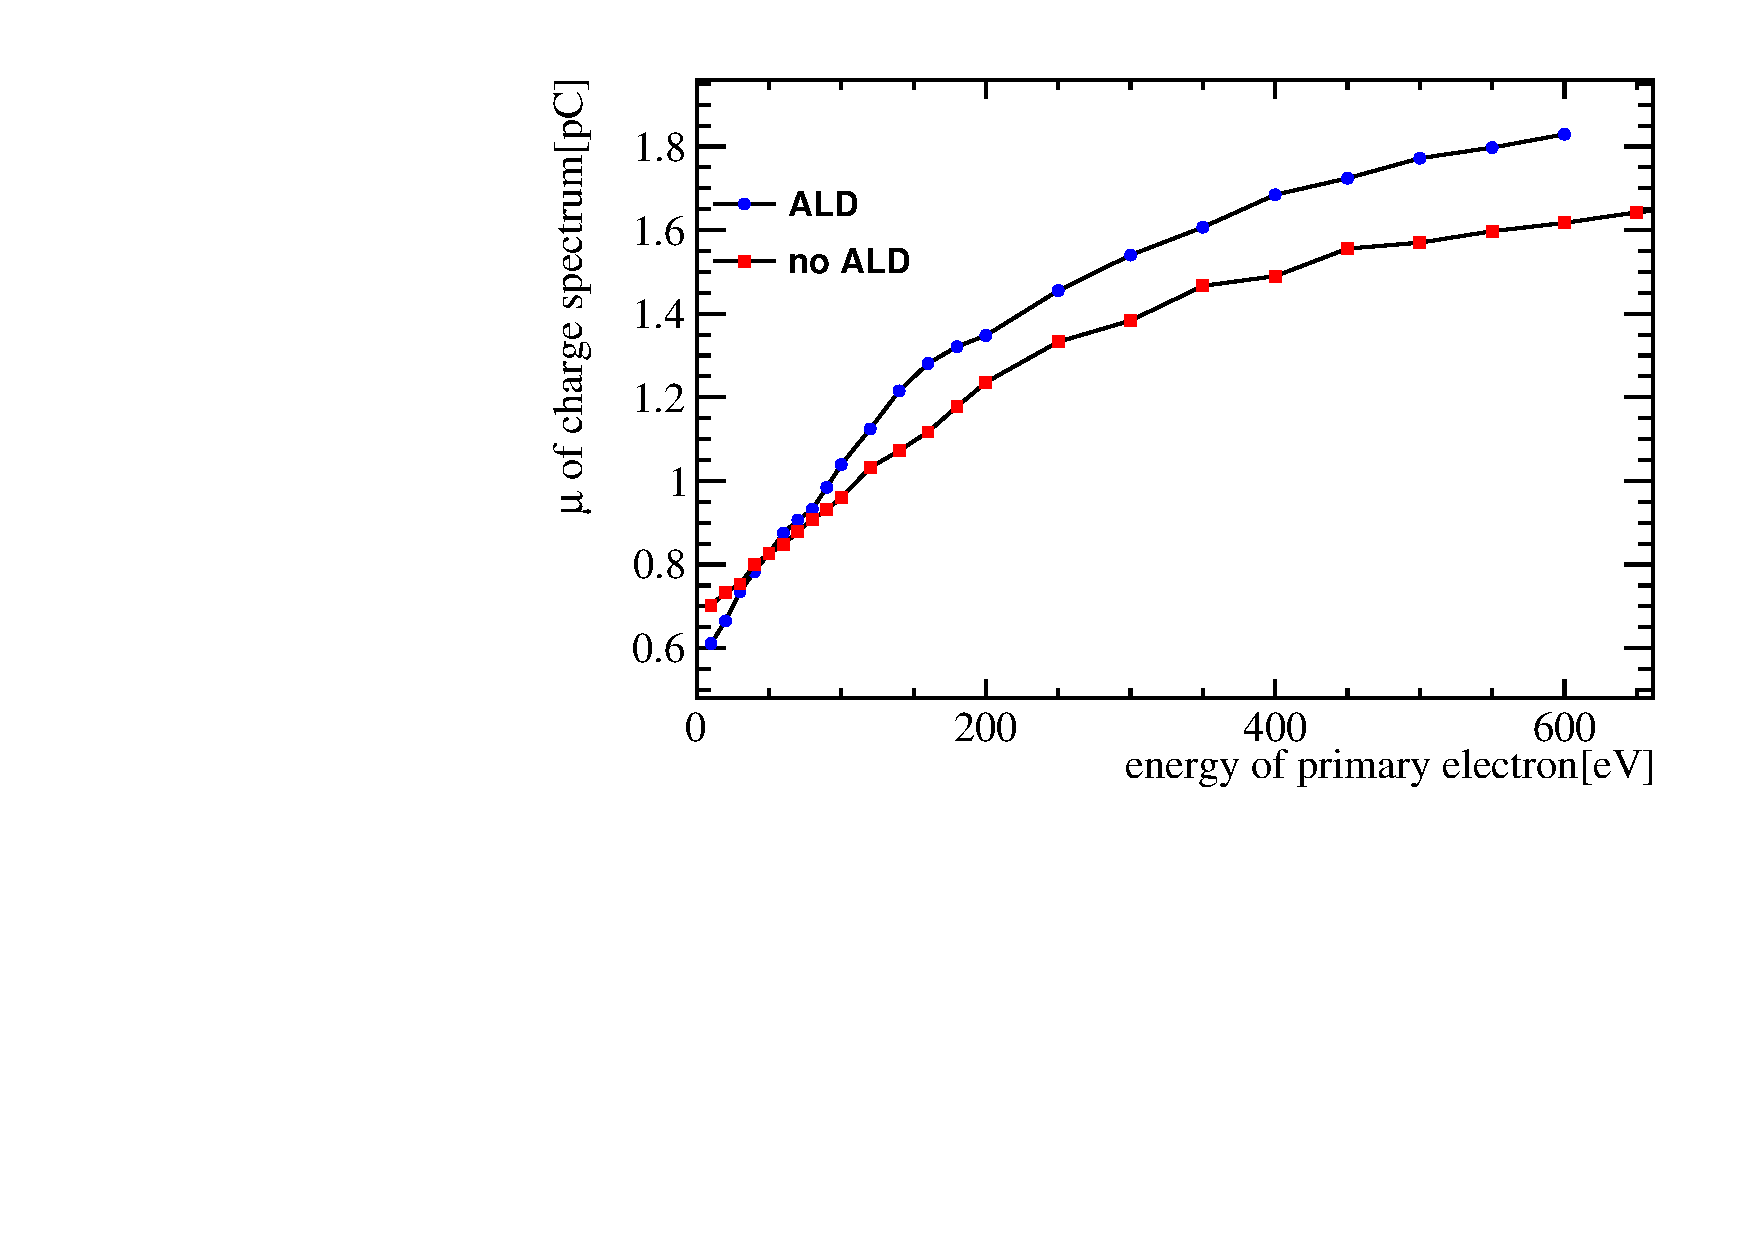
\includegraphics[width=\textwidth]{pic/gain.h5_mu.pdf}
        \caption{the mu of charge spectrum changes with the change of primary electron energy}
        \label{fig:gain}
    \end{subfigure}
    \begin{subfigure}[b]{0.45\textwidth}
        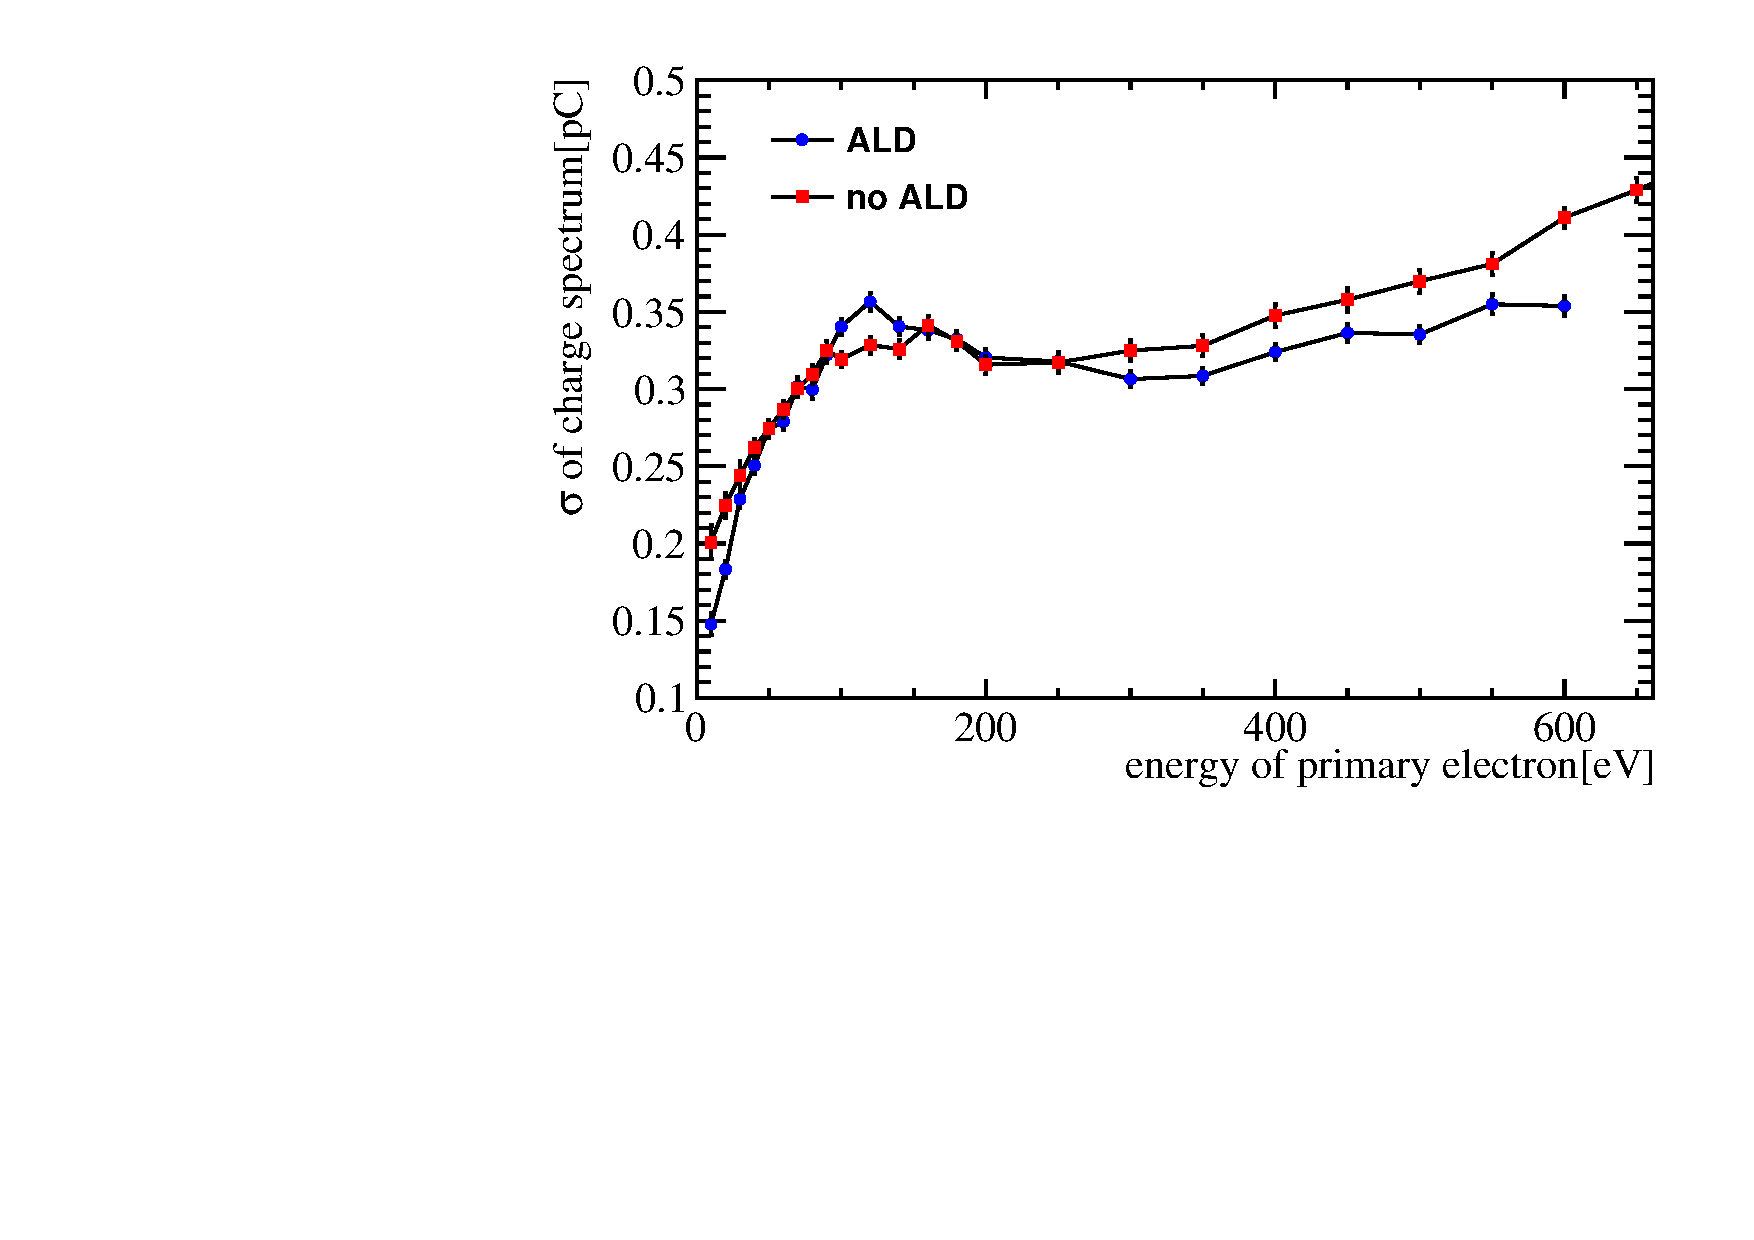
\includegraphics[width=\textwidth]{pic/gain.h5_sigma.pdf}
        \caption{the $\sigma$ of charge spectrum changes with the change of primary electron energy}
        \label{fig:sigma}
    \end{subfigure}
    \caption{mu and $\sigma$ }
    \label{fig:gaintest}
\end{figure}

When the electron energy is less than \SI{400}{eV} , the gain increases with the increase of the electron energy.
As the electron energy reaches \SI{400}{eV}, the gain gradually stabilizes.
Similar results are reported in \cite{2017MCP}.
This means in surface mode one or more secondary electrons are emitted into the channels.
Because of its lower energy, the gain formed in MCP is lower and the resulting charge is smaller.
The charges from these secondary electrons pile up on top of each other at the anode, eventually forming a larger charge signal.

The corresponding charge response of electrons with different energies is superimposed
according to the probability of the energy distribution of the secondary emission electrons
to obtain the charge response of surface mode.

\subsection{Spectrum convolution}\label{sec:convolution}
By means of Monte Carlo method, the process of electron incident multiplication can be simulated,
and the charge distribution generated by a single electron incident can be obtained.
In this work, we calculate the charge distribution of a single electron incident by the following steps:
\begin{enumerate}
    \item {Depending on the probability, determine whether the electron is directly incident into the MCP channels.}
    \item {The charge generated by the electrons directly incident on the mcp channels is
          sampled directly from the Gaussian or Gamma distribution}
    \item {If the electrons are on the surface, the yield determines
          what process in the fuman model occurs on the surface.}
    \item {In addition to the true secondary emission process,
          the incident electron energy is directly extracted from the energy spectrum
          and the charge is extracted from the Gaussian or Gamma distribution according to the energy.}
    \item {For the true secondary emission process,
          firstly, the number of electrons emitted by secondary emission 
          is determined according to the Poisson distribution
          and the energies of electrons are sampled from the SES \ref{fig:SES}, 
          and then the charge is extracted from the secondary electron energy
          and added as the final charge output. }
    \item {The above process is repeated many times to obtain a histogram of the charge distribution}
\end{enumerate}

Through the above process, the charge response generated by a single electron incident is calculated. 
In fact, what can be controlled in the test process is the light intensity, 
and the number of electrons generated by light in the photocathode follows the Poisson distribution. 
Taking this process into account, the charge response can be obtained as .
\begin{figure}[ht]
    \centering
    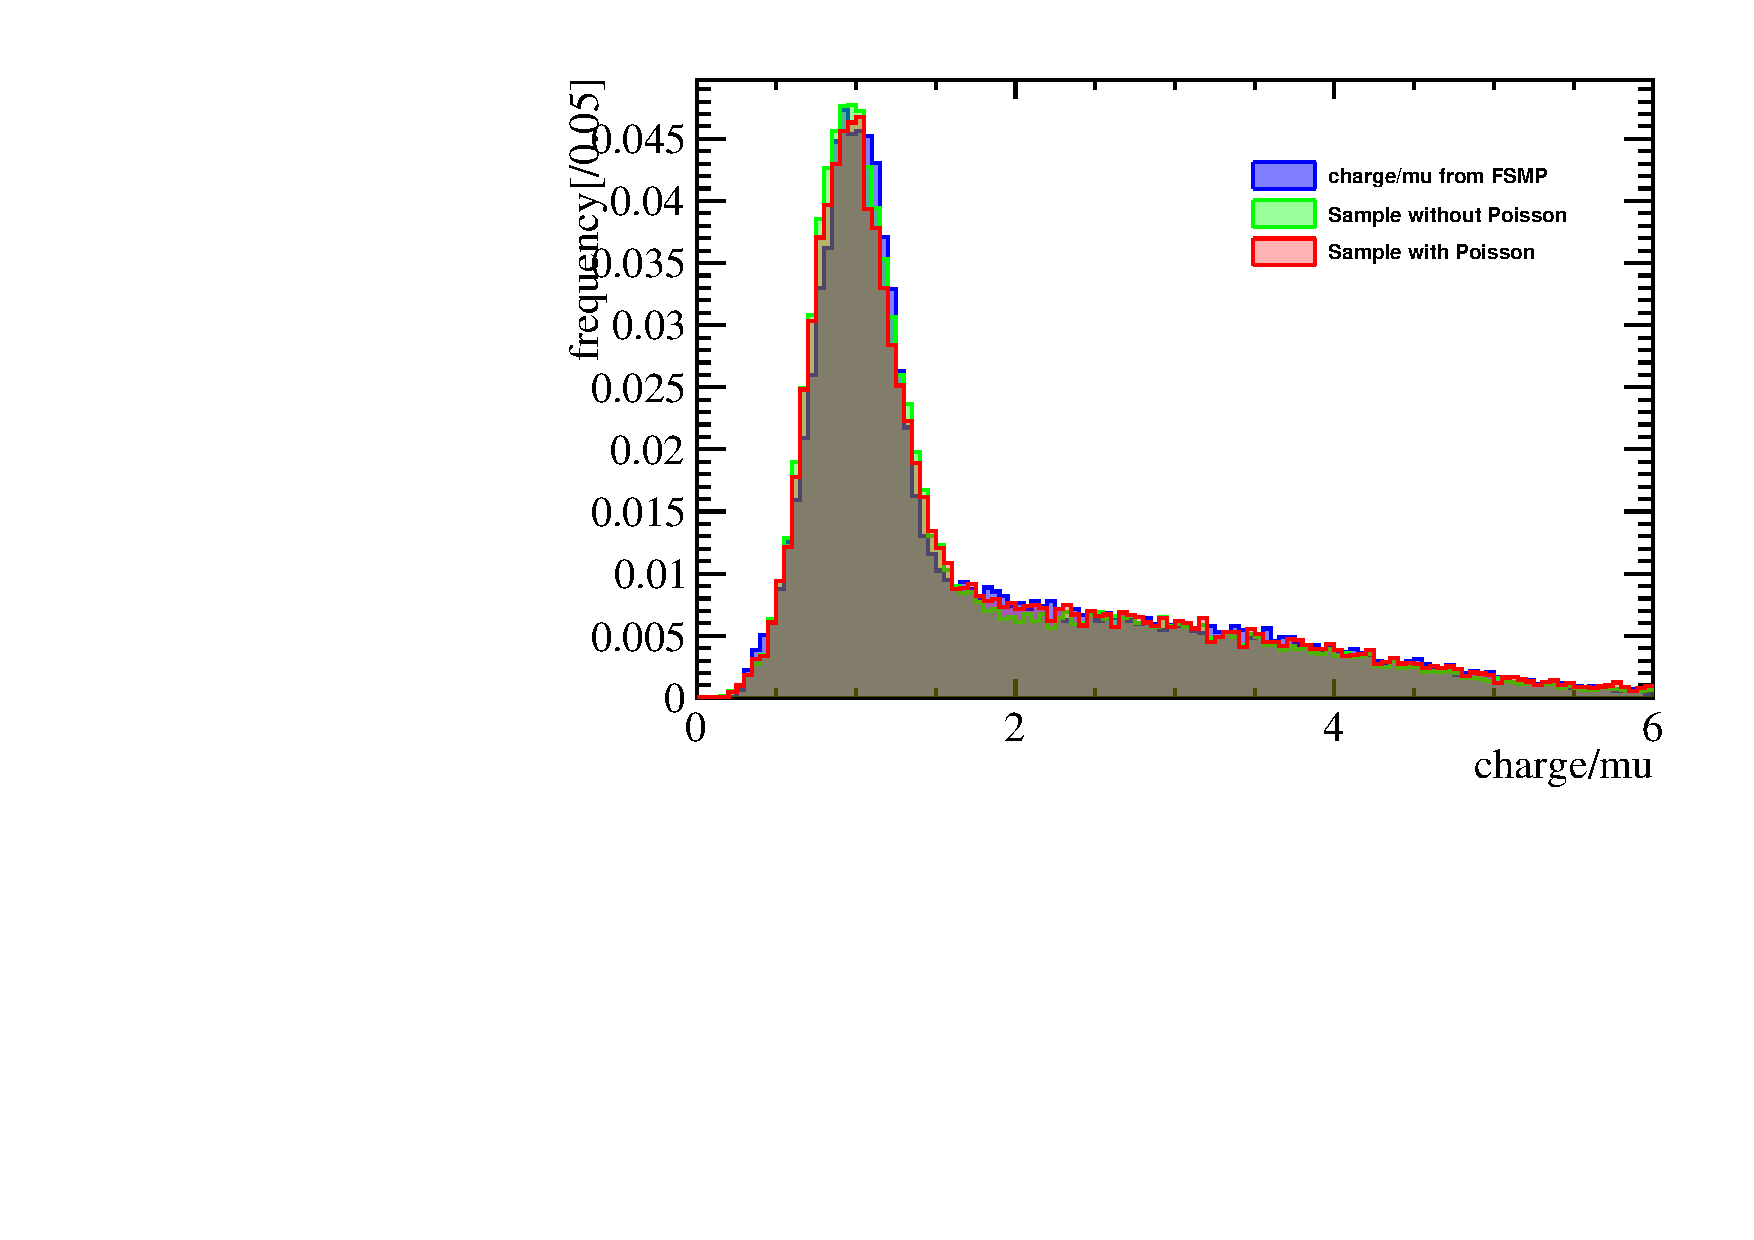
\includegraphics[width=0.6\textwidth]{pic/convolution.pdf}
    \caption{the MC charge response}\label{fig:convolution}
\end{figure}

\section{secondary electron emission affects TT distribution}\label{sec:TT}
In surface mode, Secondary electron emission from the upper surface of MCP,
and enter the channels under the influence of an electric field.
The Transit Time is delayed.

\section{Discussion and conclusion}\label{sec:conclusion}

\newpage
\bibliographystyle{plain}
\bibliography{ref}

\end{document}